\begin{figure}[H]
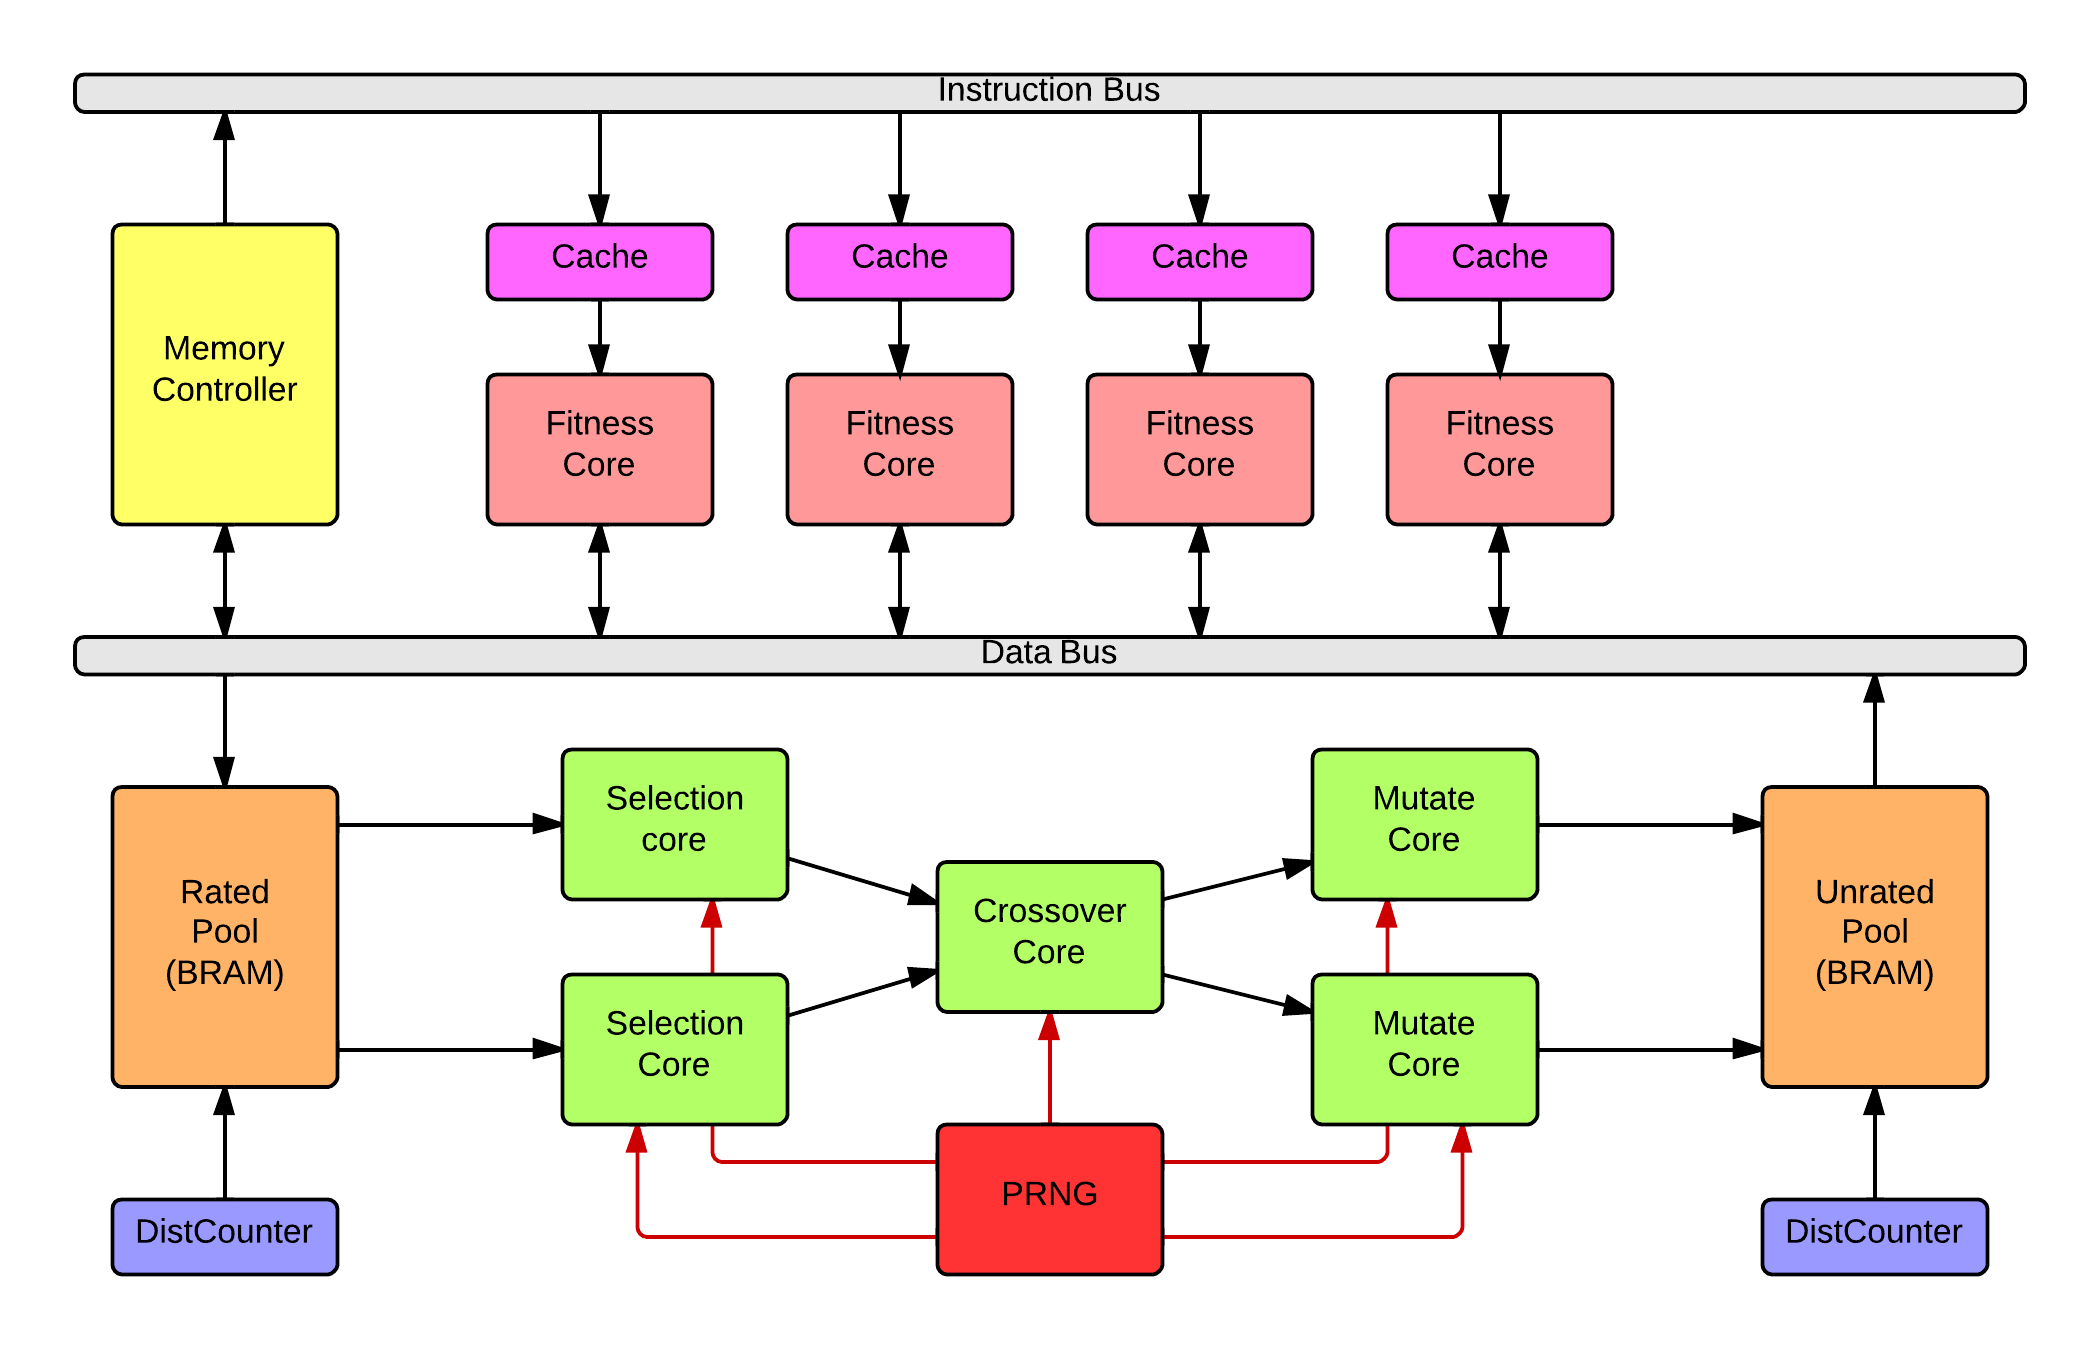
\includegraphics[width=\textwidth]{fpga/fig/processor_architecture.png}
\caption{Processor Architecture}
\label{figure:fpga-architecture}
\end{figure}

The processor architecture designed for the Barricelli computer is a very clean design, and the key to its high performance lies in its simplicity.
The architecture contains a number of general cores, which in this context are named fitness cores.
The fitness cores are general purpose cores in the sense that they are programmable and turing complete, but for genetic algorithm applications the cores are intended to calculate fitness scores of individuals.

Common genetic algorithms operations are performed by a separate hardware accelerator pipeline.
This accelerator consists of several operation-specific special cores for selection, crossover and mutation.
The fitness cores and the genetic pipeline are all connected to a single data bus.
To avoid any memory synchronization issues the data bus is controlled by a central arbitration unit.


\subsection{Instruction Memory}
\label{subsec:fpga-instruction-memory}
The \Gls{barricelli} is a \Gls{harvard machine}.
The memory is split into instruction and data memory.
This is done to achieve better memory throughput, because both memories can be accessed simultaneously.
The instruction memory is organized in a two layer memory hierarchy, with slower external memory (\gls{SRAM}) and faster, internal on-chip caches (\gls{BRAM}).
This separation combines the high instruction thoughput of fast on-board memory wit the comfortably spaceous data storage capabilities of a larger, slower chip external chip.

Each fitness core has its own private instruction memory cache which buffers instructions to decrease the number of slow memory accesses needed during runtime.
Access to an instruction cache is handled by a fitness core's dedicated cache controller, which is responsible for locating and transferring instructions from the instruction memory.
In case of a cache miss, the data-requesting core is halted until the instruction is transferred from memory.
A pseudo-algorithm describing the cache fetch operation can be found in algorithm \vref{algorithm:cache-operation}.
This scheme is created to resolve the conflicts that arise from using shared memory. 

\begin{algorithm}[H]
\SetAlgoLined
\DontPrintSemicolon
\KwData{ $ a = $ an instruction address \newline
$ Ci = $ an array of instructions \newline
$ Ca = $ an array of the corresponding addresses \newline
$ M = $ the instruction memory, indexable by instruction addresses
}
\KwResult{The instruction at address $ a $}
\Begin{
    \If{$ a = Ca[A \bmod{512}] $}{
        \Return{$ Ci[A \bmod{512}] $}
    }\Else{
        $ Caa \bmod{512}] \longleftarrow a $\;
        $ Ci[a \bmod{512}] \longleftarrow M[a] $\;
        \Return{$ Ci[A \bmod{512}] $}
    }
}
\caption{Fetching an instruction from the cache}
\label{algorithm:cache-operation}
\end{algorithm}


\subsection{Data Memory}
\label{subsec:fpga-data-memory}
The \gls{galapagos} architecture is a \gls{MIMD} architecture with shared memory.
In the \Gls{barricelli} computer, a central memory controller is responsible for synchronizing memory access on the shared data bus.
Each component that wants to access memory must go through the memory controller, and follow the proper memory access request protocol.
The controller is constructed in a way that only allows one fitness core to be able to carry out a memory request at a single time.
In case of multiple memory requests, the controller performs a selection deciding in which order the requesting cores is granted the bus.
The precise technique of selection can be seen in algorithm \ref{algorithm:round-robin-selection}.
This may introduce a potential bottleneck for memory-bound problems.
For this reason, each fitness core has a generous 31 general purpose registers, which should reduce the data memory load quite a bit.

\begin{figure}[H]
\begin{algorithm}[H]
\SetAlgoLined
\DontPrintSemicolon
\KwData{$ Requests = $ requests signals from the fitness cores\newline 
$ Request = $ 2-bits specifying the operation}
\Begin{
    $ Requests \longleftarrow $ requests from the fitness cores\;
    \While{$ True $}{
        \For {request in Requests} {
            \If{request $=$ asserted}{
                performMemoryOperation()
            }
        }
        
    }
}
\caption{Round-robin selection}
\label{algorithm:round-robin-selection}
\end{algorithm}
\end{figure}


The selection algorithm is based on round-robin scheduling, and will be explained in further detail here.
The request signals of \emph{fitness cores} are checked in turn to check if one of the cores has requested the memory bus.
The type of request is determined by combination of two request signals sent by each \emph{fitness core}.
The signals refer to either a \emph{NOP}, \emph{READ}, or \emph{WRITE} operation.
In case of \emph{NOP}, the algorithm moves on to check the next state request lines.
It continues doing this in this fashion until a \emph{READ} or \emph{WRITE} request is encountered. 

When a \emph{READ} or \emph{WRITE} operation is encountered, the \emph{data controller} starts to carry out the request from the fitness core.
Performing a memory operation takes at least four cycles, as the processor word size is 64 bits, while the memory bus to the external memory chips are only 16 bits wide.
Because of this, data needs to be shuffled across the bus 16-bits at a time, which accounts for the four cycle minimum for data operations.

For the external memory to be operated correctly by the memory controller, the proper control signals need to be set at the correct times. The signals required differs depending on the type of operation, \emph{READ} or \emph{WRITE}. The timing diagrams can be seen in figure \ref{fpga:fig:timing:dmem:read} and \ref{fpga:fig:timing:dmem:write}, respectively. 

\todo{Check text}

\begin{figure}[H]
  \centering
  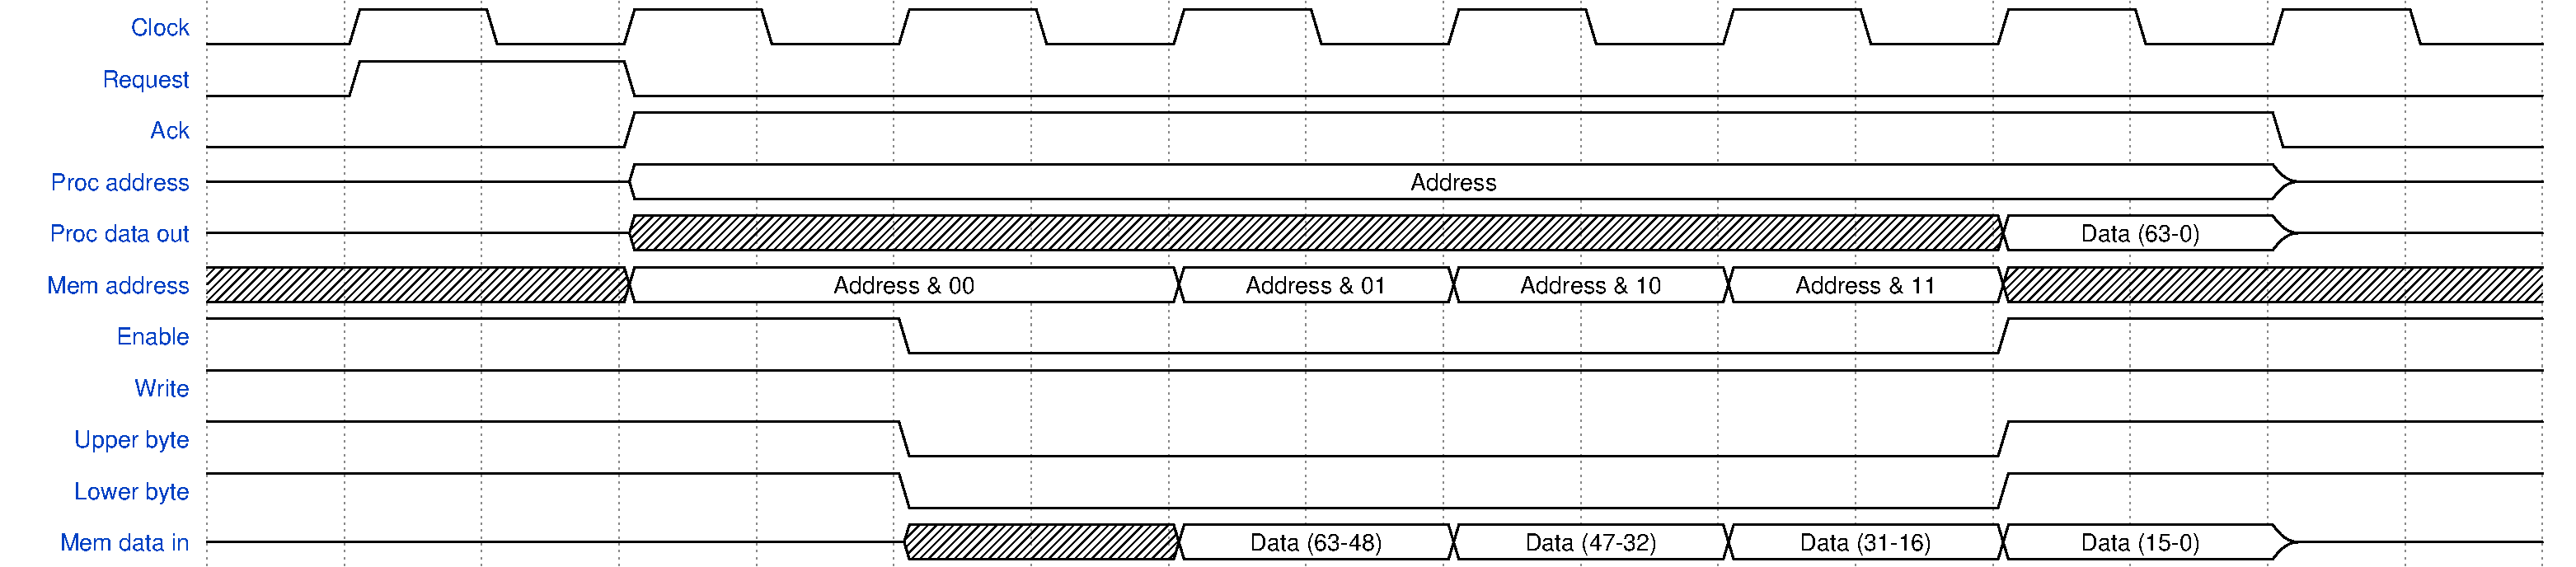
\includegraphics[width=\textwidth]{fpga/fig/timing/data_mem_read.pdf}
  \caption{Data memory read cycle}
  \label{fpga:fig:timing:dmem:read}
\end{figure}

\begin{figure}[H]
  \centering
  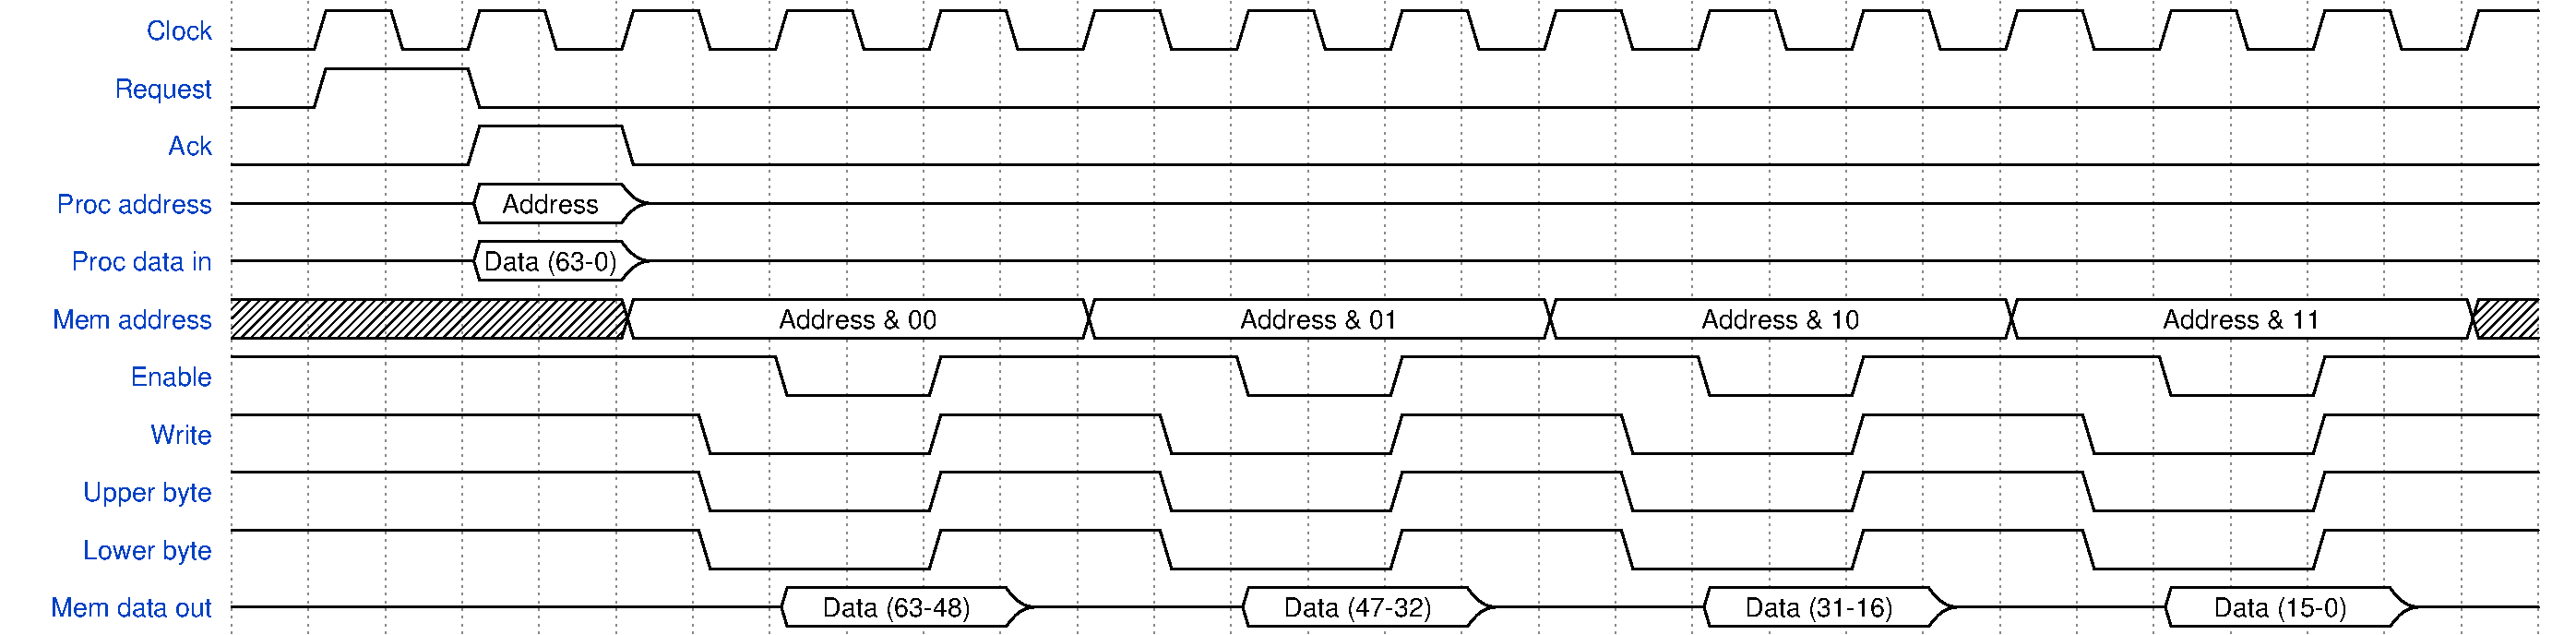
\includegraphics[width=\textwidth]{fpga/fig/timing/data_mem_write.pdf}
  \caption{Data memory write cycle}
  \label{fpga:fig:timing:dmem:write}
\end{figure}

As is immediately apparent in figures \vref{fpga:fig:timing:dmem:read} and \vref{fpga:fig:timing:dmem:write}, the number of cycles required for load and store operations are are 5 and 13 cycles, respectively.
A state machine is implemented in the \emph{data memory controller} to handle interfacing with the external memory chips.
This state machine is responsible for controlling that the different signals are set according to the diagrams.
For more detailed view of the \emph{Data memory controller}, the reader is advised to study the state machine diagram in figure \ref{fpga:fig:mem:data_memory_ctrl_state_machine} and the accompanying data path in figure \ref{fpga:fig:mem:data_memory_ctrl}.

\begin{figure}[H]
  \centering
  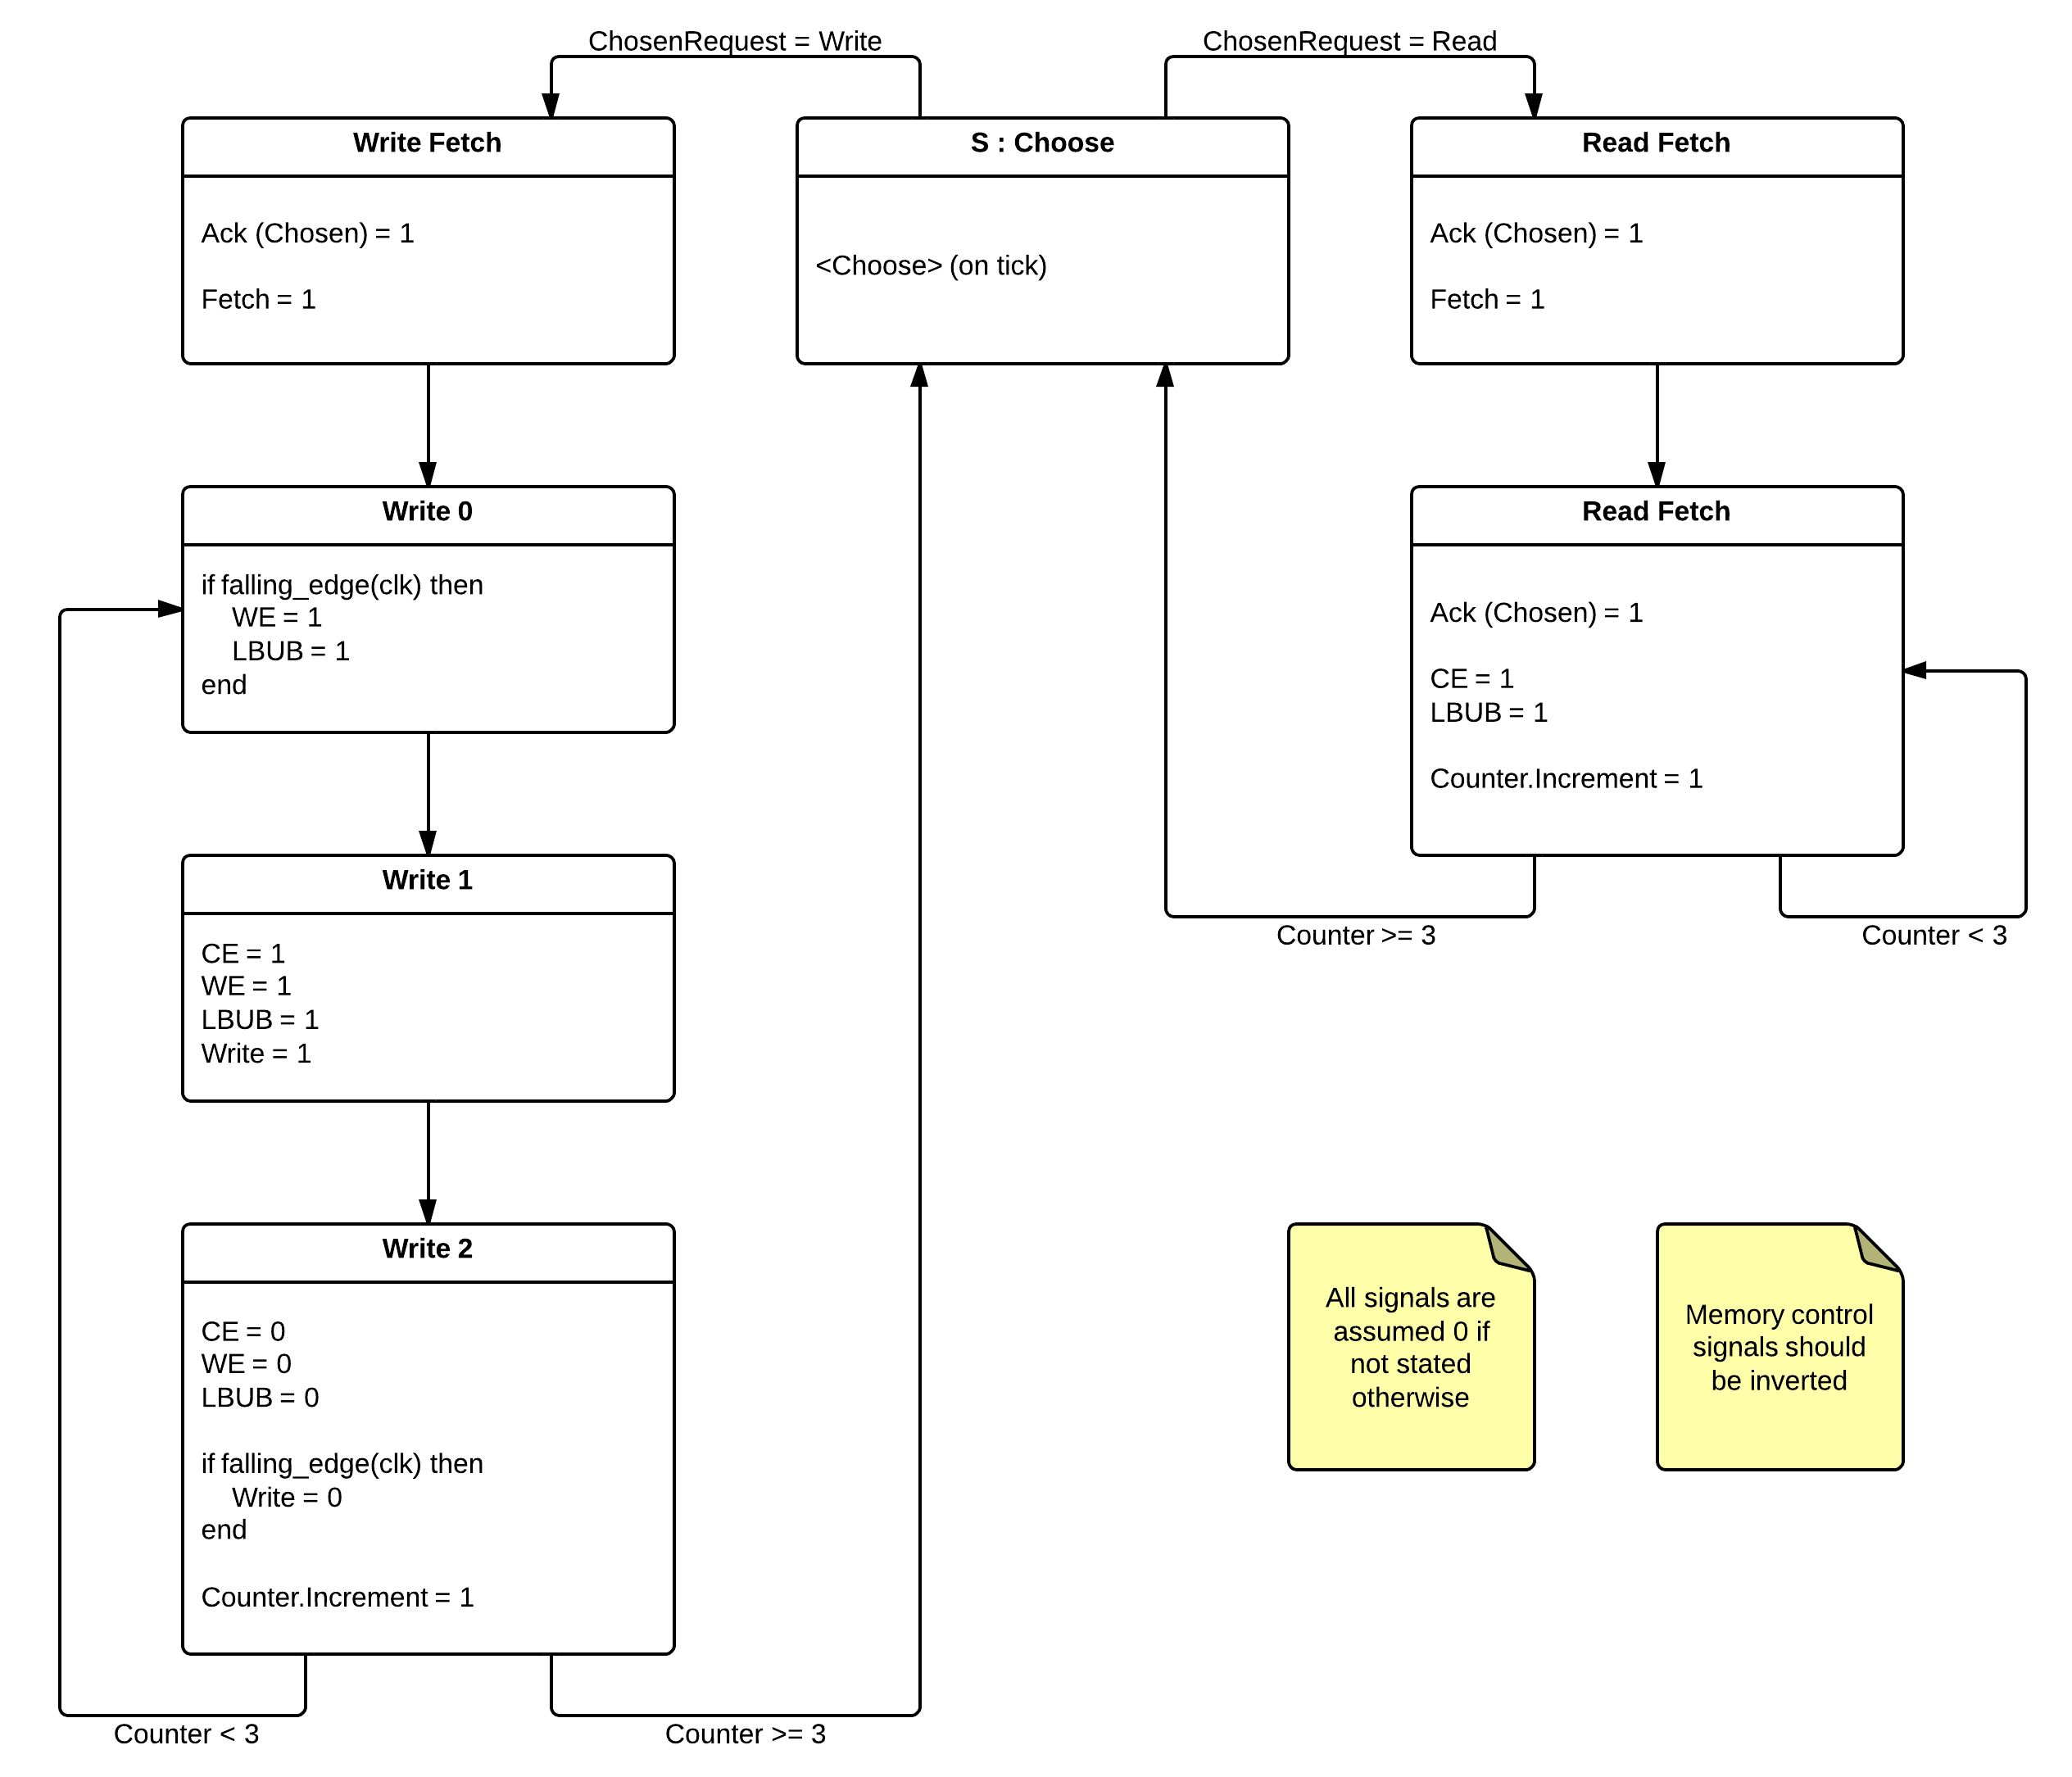
\includegraphics[width=\textwidth]{fpga/fig/memory_ctrl_state_machine.png}
  \caption{Data memory controller state machine}
  \label{fpga:fig:mem:data_memory_ctrl_state_machine}
\end{figure}


\begin{figure}[H]
  \centering
  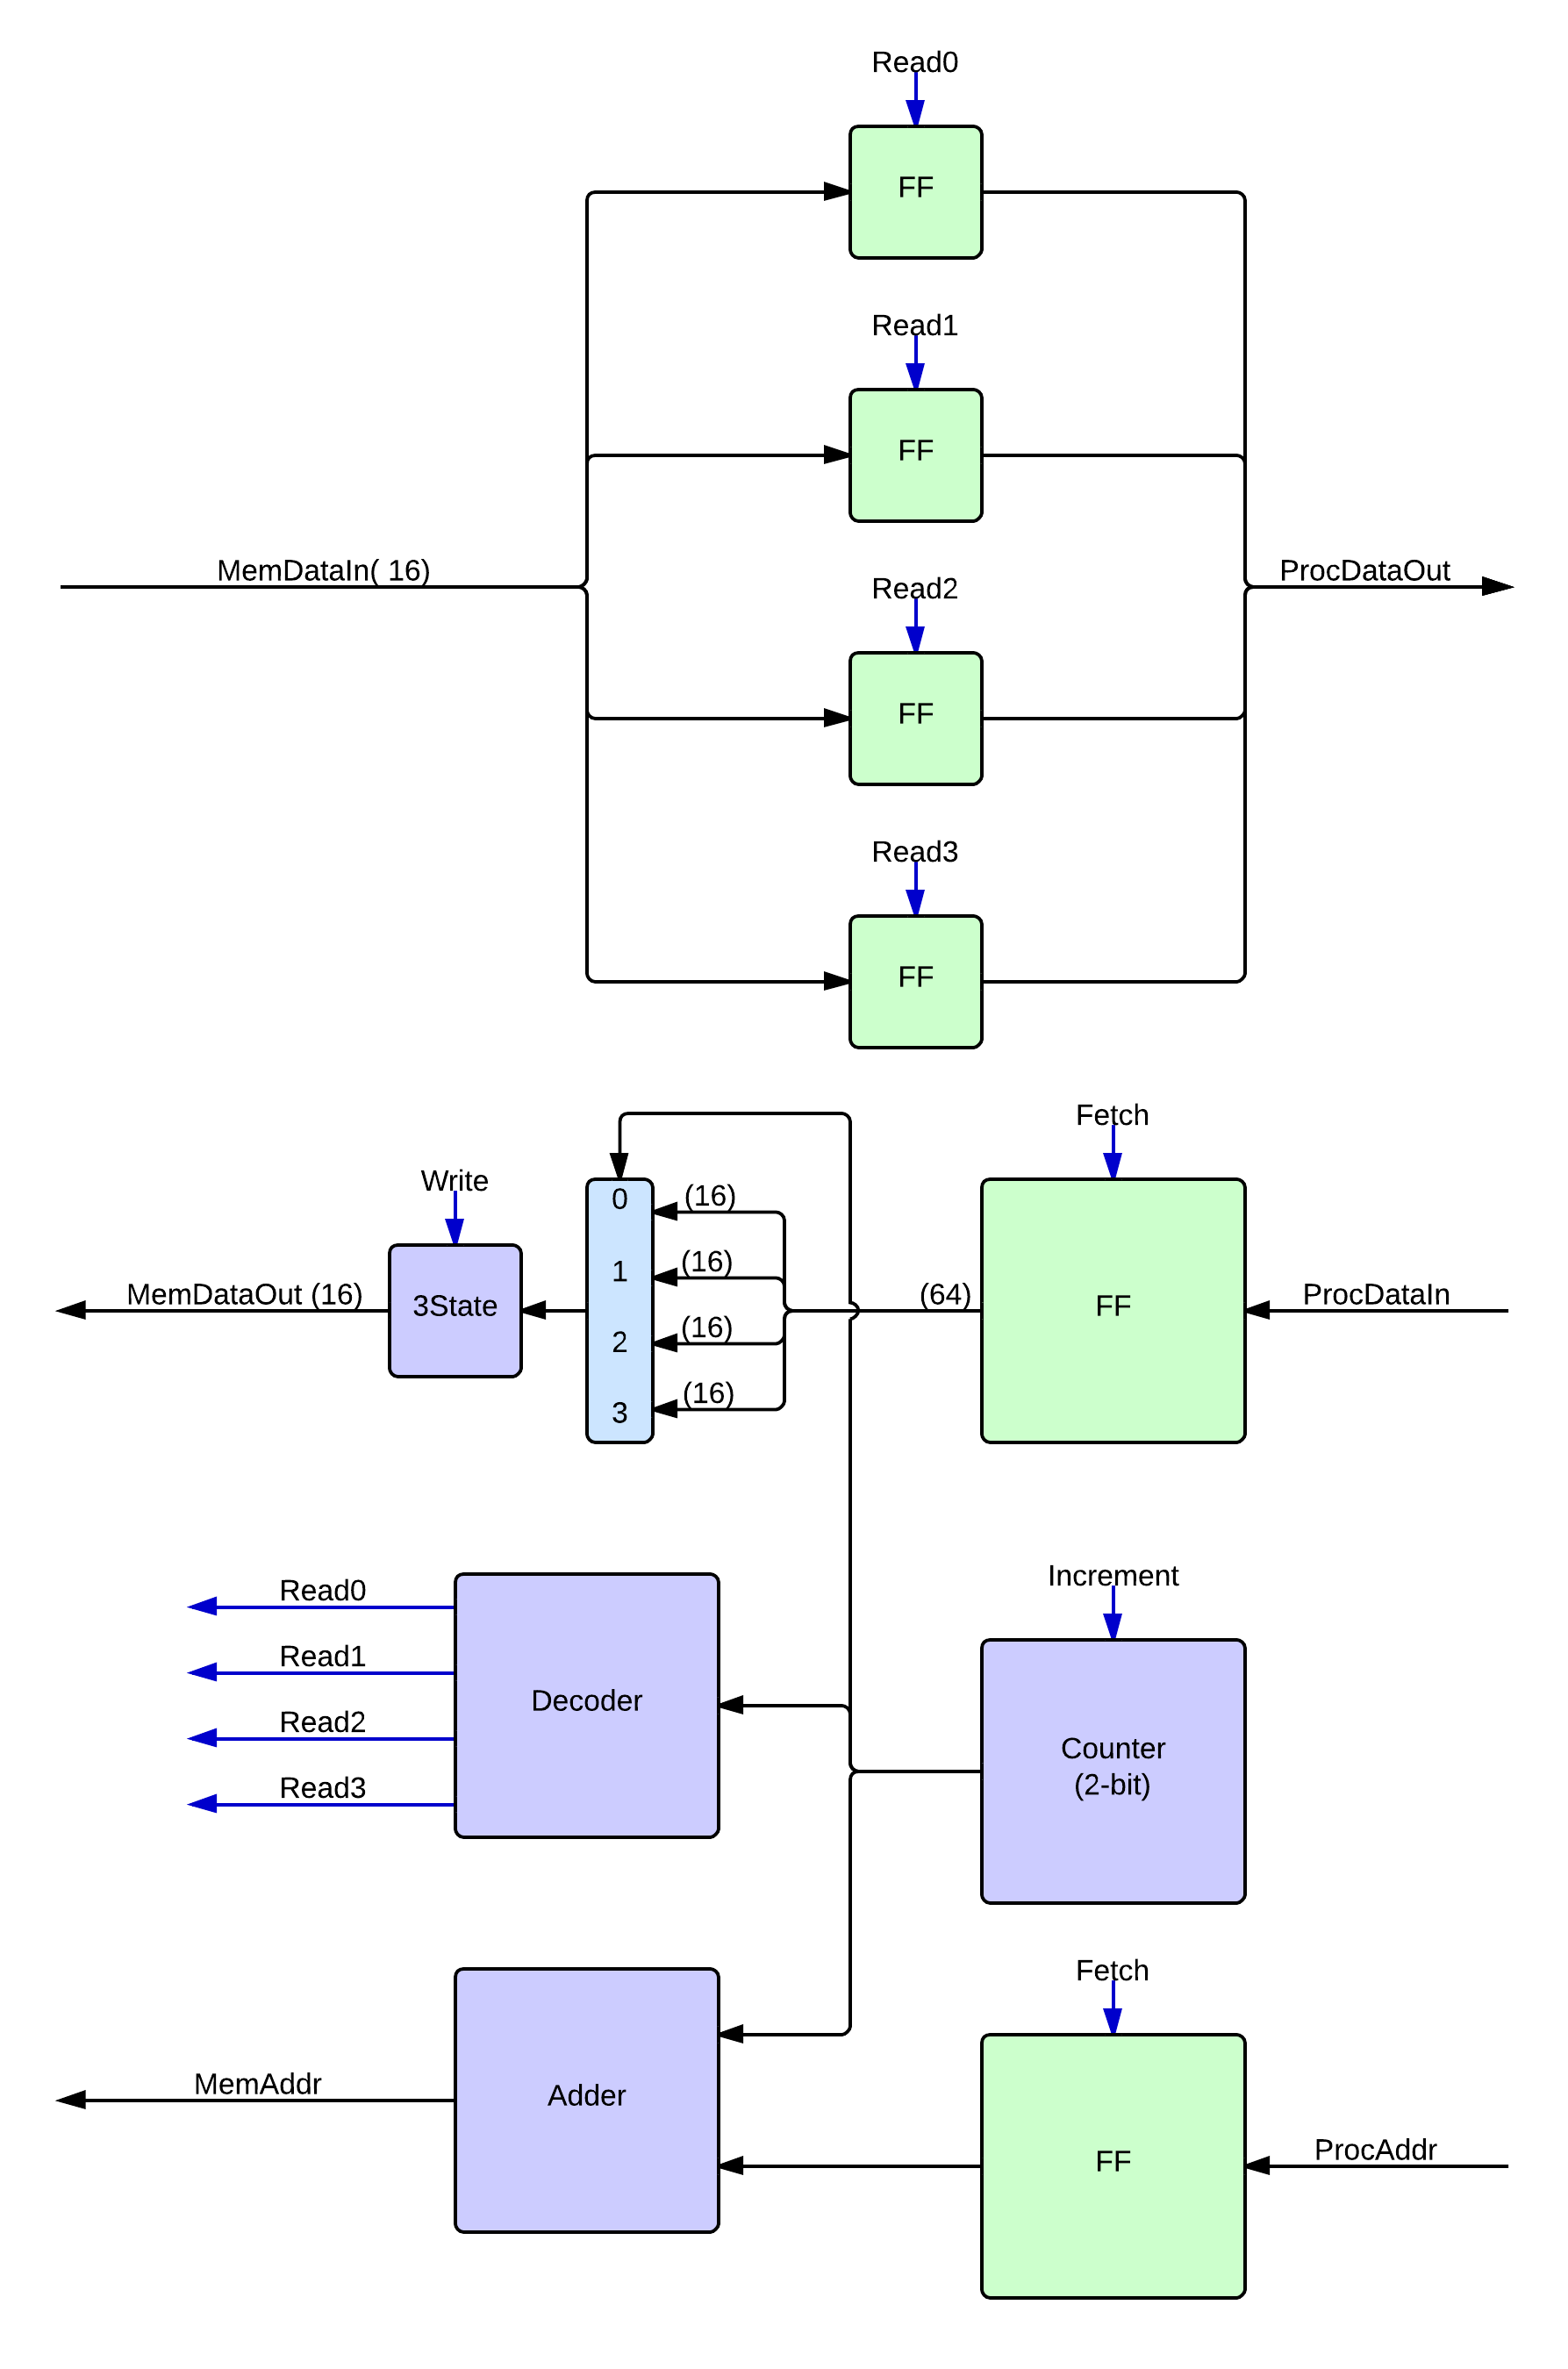
\includegraphics[width=\textwidth]{fpga/fig/memory_ctrl.png}
  \caption{Data memory controller signals mapping}
  \label{fpga:fig:mem:data_memory_ctrl}
\end{figure}


\todo{write about and ref to above graphs}


\subsection{Rated and Unrated Pools}
Individuals making up the populations are stored on the FPGA for for faster access. These are stored in \emph{BRAM} on the FPGA. This implies a lot faster access times, compared to access times to the external memory, as mentioned in (?). This is done to achieve better memory throughput when executing the algorithms. The pools are further divided into two separate \emph{BRAM} blocks, one for rated individuals, and one for un-rated. This is done to achieve even better memory throughput. The increased throughput are achieved because the different computational can work on the rated and un-rated pool simultaneously. For instance while one fitness core is storing a ranked individual, while another fitness core is fetching a new individual for ranking. 

\todo{More details and better explanation} 

Both the rated pool and the unrated pool is associated with the a controller, referred as the \emph{Genetic controller}. As with the data controller, this controller is responsible for granting access for the rated and unrated pool. This buses in question are, however, not the same as those used to access the data memory. The genetic controller use their own separate buses. The controller is based on mostly the same idea as the data controller described in section (?). The when performing genetic operations, the fitness cores need to request the data bus by using two request signals. The combination of these signals refer to the operation the fitness core requests from the genetic controller. 

The genetic cores continuously performs a round-robin in order to grant bus to the requesting fitness core. The logic surrounding the different operations are implemented as an state machine to divide the operations in different clock cycles. This is the same method as used in the data controller.







The state machine can be seen in figure(?)




\subsection{PRNG Module}
The genetic algorithms need diversity in the search space in order to be able to converge to a solution. To achieve this, the architecture need some way of creating sufficiently random numbers. These generated numbers do not need to be true randoms number, this implies that a psudo number generator will suffice. 

    
 

\subsection{Fitness Core} \label{fpga:fitness:ss:design_of_the_fitness_core}
    \subsection{Design of fitness core}

The design of the fitness core is highly influenced by MIPS.
The core is designed as a five stage pipeline.
The goal is to make it as simple as possible, and at the same time harvest efficiency by instruction level parallelism.
The more advanced features like branch prediction and instruction scheduling are not taken into consideration while designing the CPU.
The hazard detection schemes will be made simple.
The hazard resolutions will be made in software as well as in hardware.
The plan is to simply stall when we encounter any hazards in the pipeline.
The assembler will handle the most obvious ones to achieve efficiency, while the hardware will simply stall when hazards are detected.

\fxnote {The hazard scheme may change if time}
 \label{fpga:subsection:fitness_core}


\subsection{The Genetic Pipeline}
\label{fpga:subsection:genetic_pipeline}
\todo{some words about the genetics accelerator}
The galapagos architecture includes a highly specialised pipeline for performing genetic operations. The pipeline is based on the observation that selection, crossover, and mutation works similar for a specific subset of problems. These can therefore be implemented as hardware accelerators constructed for performing one specific task. Constructing such accelerators has been proven to be very beneficial regarding performance. Designing specialised hardware is usually simpler and thereby more effective than constructing general purpose components.\todo{Bullshit ?} This pipeline will effectively relieve the general cores, the fitness cores, from computing the evolution of individuals. The idea is that these will make the fitness cores able to only focus on the computation of fitness ranking, which is considered computational intensive. In the mean time the \emph{genetic pipeline} can produce new data for ranking. These operations could have been performed by the processor, however, the processor is badly suited for these kind of operations. Note that the instructions in the pipeline actually uses 5 cycles in order to complete propagate through the pipeline. It is a far better to only use one cycle in order to complete the one specific operation.  

The genetic pipeline is constructed with three specialised cores for performing selection, crossover, and mutation. These are operations that occurs frequently in genetic algorithms. These are connected to two internal memory banks on the \emph{FPGA}, namely the unrated and rated pool.


-Abstraction for the programmer. Simpler to program.
-Do not need components like ALU
- effective 
- Less control over the genetic pipeline
- 



\subsubsection {Selection Core} \label{fpga:selection:ss:selection_core}
    \subsection {Design of the selection core} \label{fpga:selection:ss:selection_core}

The selection core is designed based on a tournament selection algorithm. It is designed to select an chromosome from a random position in the rated pool. The current best and the random selected is compared to each other with use of an comparator. The best chromosome is stored and used in the next tournament round. After some number of tournaments the current best is transferred to the crossover core. The selection core is actually responsible for letting the rest of the genetic pipeline know when it can fetch the next chromosome. 

The selection core is designed with efficiency in mind. The overall time spent in the genetic pipeline must be smaller than the time spent ranking the chromosomes. Note that the fitness cores are connected to the same memory bus as the genetic pipeline. This could potentially lead to a memory bottleneck resulting in starvation. The selection core tries to overcome this fact by reducing the memory access to a minimum. Note that the selection core has reserved the memory bus during the ongoing tournament. This implies that port used by the selection core is unavailable to others during this time. It is designed to not use the memory more than it absolutely have to. For instance, if the current fitness value is greater than the fitness value just fetched. The selection core will not bother fetching the accompanying chromosome. Ensuring that the memory resources are not wasted. This is accomplished with an \emph{state machine}. 



\subsubsection{Data Path}
Upon the beginning of the data path design, the group wanted to determine the the components required to perform the selection. In this specific case the group decided to design a data path able to perform a tournament selection. The resulting architecture is made as simple as possible.  It is composed of \emph{flip flops}, \emph{control unit} and an \emph{comparator}. The different components are connected as seen in figure.




\fxnote{Add figure of selection core}


\subsubsection{Control Unit} \label{fpga:selection:sss:control_unit}



\subsubsection {Comparator} \label{fpga:selection:sss:comparator}



\subsubsection{Case study} \label{fpga:selection:sss:case_study}



 \label{fpga:subsection:selection_core}

\subsubsection{Crossover Core} \label{fpga:crossover:ss:crossover_core}
    The crossover Core is the next part in the genetics accelerator after the selection cores. Two inputs are forwarded from the two selections cores as "parents", and two outputs are the "children" of the inputs, containing bits from both parents. All the bits from both the parents are forwarded in the children, but in some parts the bit-patterns are switched on the children, based a selected crossover function and on a random input from the PRNG. Henceforth this is called crossover.

There are three distinct crossover functions that are implented: Split, doublesplit and function.

\paragraph{\textit{Split Fucntion}}
\begin{figure}[H]
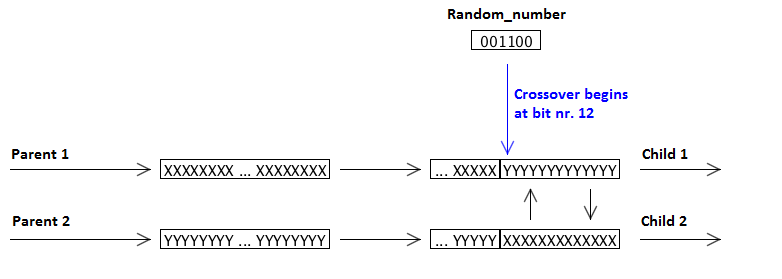
\includegraphics[width=\textwidth]{fpga/fig/crossover_split.png}
\caption{Crossover split function}
\label{fig_crossover_split}
\end{figure}

The first function, crossover split, performs crossover from a selected bit number in the children and until the edge (bit number 0). This can be seen in figure \ref{fig_crossover_split}. The values in the parents are represented with X's and Y's, and a single X or Y can have the value 0 or 1, independent of each other.
The bit number for starting crossover is based on the value of a 6-bit input random\_number, which is provided by the PRNG. This value ranges from 0 to 63.

\todo Describe how it technically works??

\paragraph{\textit{Double-split Fucntion}}
\begin{figure}[H]
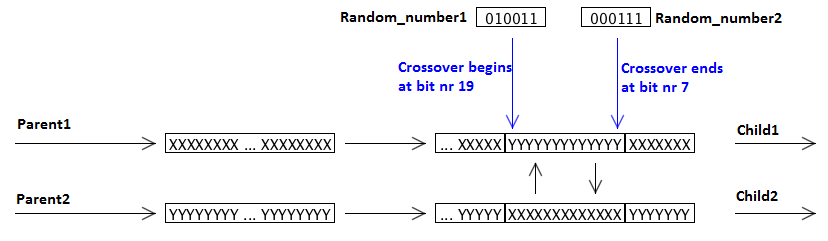
\includegraphics[width=\textwidth]{fpga/fig/crossover_doublesplit.png}
\caption{Crossover double-split function}
\label{fig_crossover_doublesplit}
\end{figure}

The second function, crossover double-split, is similar to the crossover\_split-function, but in additionally to having a starting bit for crossover, it also has an ending bit where the crossover starts, instead of reaching the edge at bit nr. 0. PRNG provides with 2 6-bit inputs, random\_number1 and random\_number2, whose values selects the starting bit and the ending bit for the crossover. These values range from 0 to 63, and if both are the same, then only one bit will be selected for crossover.

\todo Describe how it technically works??

\paragraph{\textit{XOR Fucntion}}
\begin{figure}[H]
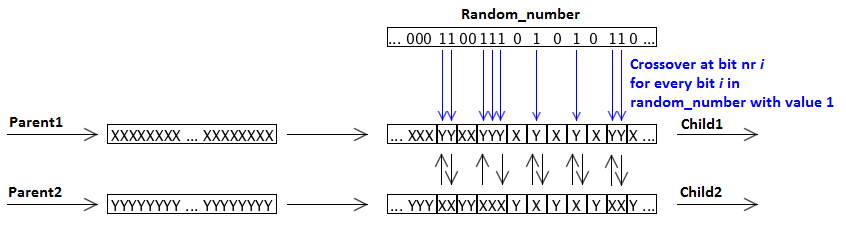
\includegraphics[width=\textwidth]{fpga/fig/crossover_xor.png}
\caption{Crossover XOR function}
\label{fig_crossover_xor}
\end{figure}

The third function, crossover XOR, performs crossover bit by bit, based on the 64-bit input random\_number. For each bit number \textit{i} in random\_number that has the value 1, the function will perform crossover on the children at the same bit number \textit{i}. This function is called XOR because of use of XOR-gates in earlier version of the function, and the principle is still the same: For each bit number \textit{i} in the child, the value will the bit number \textit{i} from one and only one parent. And which parent it is depends on the value of bit number \textit{i} in random\_number.

\todo Describe how it technically works??

\paragraph{\textit{Crossover Core Toplevel}}

The crossover core is implemented on the genetics accelerator as a toplevel containing 3 subcores, one for each function, as well as a fourth path with no crossover. In addition to the two parent inputs and 64-bit input random\_number, the toplevel has a control\_number input used for determining which crossover function is to be used: Split, doublesplit, xor, "party mode" or no crossover at all. Party mode is choosing crossover function at random, based on the 2 LS bits in the random\_number. In this way, whenever inputs are sent through the crossover\_toplevel, different functions may be used at different times. These are the control values:
\begin{itemize}
\item 000 - Split
\item 001 - Double-split
\item 010 - XOR
\item 011 - No crossover
\item 1XX - Party mode, in which case these are the random control values:
    \begin{itemize}
    \item 00 - Split
    \item 01 - Doublesplit
    \item 10 - XOR
    \item 11 - No crossover
    \end{itemize}
\end{itemize} \label{fpga:subsection:crossover_core}

\subsubsection{Mutation Core}\label{fpga:mutation:ss:mutation_core}
    The mutation core is the final part in the genetics accelerator. The mutation core takes in a forwarded child from the crossover core as input and may perform mutation on a few selected bits before passing on the result. 

\begin{figure}[H]
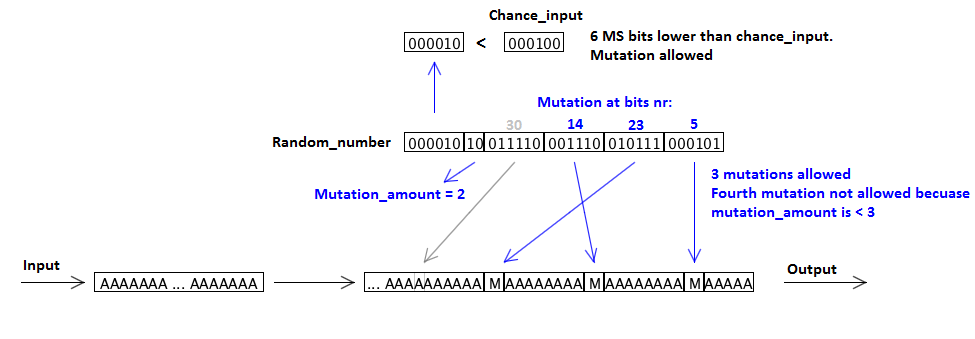
\includegraphics[width=\textwidth]{fpga/fig/mutation.png}
\caption{Mutation core function concept}
\label{Fig_Mutation}
\end{figure}

In addition to the the 64-bit child, the mutation core also takes in a 32-bit random\_number and a 6-bit chance\_input as inputs. As it can be seen in the example in figure \ref{Fig_Mutation}, all bits that are not mutated are represented by an A, and mutated bits are represented with M. The values in each A or M can be 0 or 1, independent of each other. The value M at bit number \emph{i} is the opposite of the original value A at same bit number \emph{i} in the input.
The 6 first bits in the random\_number is compared to the chance\_input, and mutation happens only if the value of these bits are less than the chance input. For each different value in chance\_input, the user may increase or decrease the chance of mutation by about 1,5\%, or $(1 / 2^6)$. If the chance input is set to 000000, no mutation will ever happen, and the user may in this way disable the mutation core.

The next two bits in the random number (bits 25-24) are used to determine how many mutations will happen. There are 4 different values, therefore there can be 1-4 mutations.
The next 24 bits are used to determine which bits are to be mutated. 6 bits are used for finding each bit number. This is similar to what is done in the split and doublesplit functions in the crossover core. These values are numbered, representing their bit field:
\begin{itemize}
\item Nr. 1: 5-0
\item Nr. 2: 11-6
\item Nr. 3: 17-12
\item Nr. 4: 23-18
\end{itemize}
These are numbered after the amount of allowed mutation. Nr. 1 will always happen when a mutation occurs, while nr. 4 happens only when the amount\_number allows for 4 mutations.

Note that if more than one of these numbers point to the same bit to be mutated, the output M will still be the inverted from the original input. For instance, if both numbers 1 and 2 (bits 11-6 and 5-0) have the value 000110, and therefore point at bit number 6, the same mutation will still happen as if only one of these numbers were 000110. If the input bit was 1, the mutated will be 0, and vice versa.
In the example provided in figure \ref{Fig_Mutation}, the 6 first bits of the random\_number are less than the chance\_input, therefore a mutation happens. Bits 23-0 have the values 30, 14, 23 and 5. Because the value of bits 25-24 is 10 (mutation\_amount has value 2), there will be 3 mutations, and the fourth does not occur (though the figure shows where it would have occured if allowed).

\begin{figure}[H]
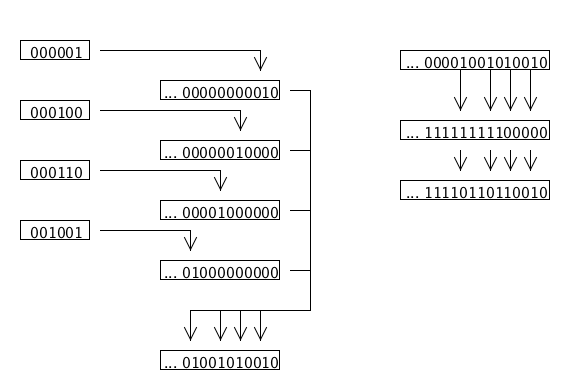
\includegraphics[width=\textwidth]{fpga/fig/mutation_mask.png}
\caption{Setting mutation}
\label{fig_mutation_mask}
\end{figure}

The mutation core is implemented by use of four shifter variables, one for each possible mutation, and set so that only one bit is 1 for the output. A final mutation is set by combining the outputs from the shifter variables by using OR-funftion, and the mutation\_amount determines how many of these outputs are combined. Figure \ref{fig_mutation_mask} shows an example where bits 1, 4, 6 and 9 are set for mutation. In this case the final output is set by combining the input and mutation with the XOR-fuction, so that for each bit \emph{i}, the bit is set to 1 if and only if bit \emph{i} is set in either the input or the mutation, but not both. This can be seen in figure \ref{fig_mutation_perform}.

\begin{figure}[H]
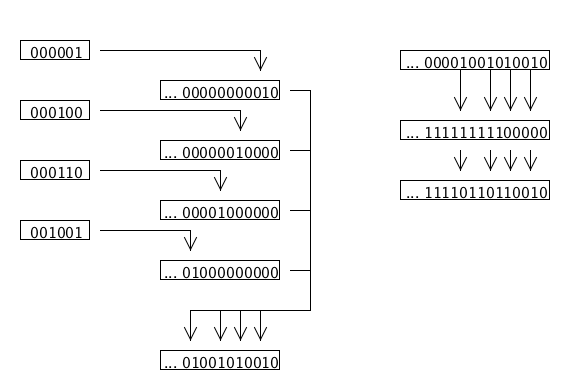
\includegraphics[width=\textwidth]{fpga/fig/mutation_mask.png}
\caption{Performing mutation}
\label{fig_mutation_perform}
\end{figure}

\todo{ "Selected bit number" needs to somehow be defined in the description of the shifter variable + ShifterVariable needs to be described.} \label{fpga:subsection:mutation_core}




\subsection{Parallelism}
\todo{awkwardly placed section.. move it somewhere else?}
The Barricelli is a MIMD computer, which means that it can execute multiple different instruction streams on multiple different data streams simultaneously, in parallel.
The four\cn fitness cores in the archtecture have each their own program counters and may load different data independantly of eachother.
They all share the same data and instruction memory, however, which makes the Barricelli a shared memory model MIMD computer.
Additionally, the genetic pipeline contains multiple specialized cores, which can also execute independant, less general instruction streams on independant data.

